% =============================================================================
% Retrieval Asymmetry in PHI-Tokenized Vector Stores
% Target: medRxiv preprint, eventual JAMIA submission
% Authors: Udit <first-author>, [co-authors TBD]
% Final v0.2: refined manuscript merged with bootstrap eval results (2026-05-23)
% =============================================================================
\documentclass[11pt,a4paper]{article}

\usepackage[utf8]{inputenc}
\usepackage[T1]{fontenc}
\usepackage{lmodern}
\usepackage[margin=1in]{geometry}
\usepackage{microtype}
\usepackage{graphicx}
\usepackage{booktabs}
\usepackage{array}
\usepackage{hyperref}
\usepackage{authblk}
\usepackage{xcolor}
\usepackage{listings}
\usepackage{amsmath}
\usepackage{caption}
\usepackage{titlesec}

\hypersetup{
  colorlinks=true,
  linkcolor=black,
  urlcolor=blue!60!black,
  citecolor=blue!60!black
}

\lstset{
  basicstyle=\ttfamily\footnotesize,
  breaklines=true,
  frame=single,
  numbers=none,
  showstringspaces=false
}

\titleformat{\section}{\large\bfseries}{\thesection}{1em}{}
\titleformat{\subsection}{\normalsize\bfseries}{\thesubsection}{1em}{}

\title{\textbf{Retrieval Asymmetry in PHI-Tokenized Vector Stores:\\
A Silent Failure Mode in Privacy-Preserving Clinical\\ Retrieval-Augmented Generation}}

\author[1]{Udit Raj \textsc{Akhouri}\thanks{Correspondence: udit@branelabs.org}}
\author[2]{[Clinical Informaticist Co-Author --- TBD]}
\author[3]{[ML / Privacy Co-Author --- TBD]}
\affil[1]{Brane Labs, Bengaluru, India}
\affil[2]{[Institution --- TBD]}
\affil[3]{[Institution --- TBD]}
\date{\today}

\begin{document}
\maketitle

% =============================================================================
\begin{abstract}
\noindent
\textbf{Background.} Retrieval-augmented generation (RAG) is increasingly
used to ground clinical large-language-model (LLM) applications in patient
records. Privacy regulations (HIPAA in the United States, GDPR in the
European Union, the Digital Personal Data Protection Act, 2023 in India)
constrain how protected health information (PHI) may be exposed to external
model providers. Two common mitigations have emerged: (i) one-way redaction
of PHI before embedding, and (ii) read-side pseudonymization, in which only
the query is tokenized while the indexed corpus retains raw identifiers.
Both are operationally attractive, yet their effect on retrieval quality has
not been systematically characterized.

\textbf{Objective.} To formalize \emph{retrieval asymmetry} --- a failure
mode in which the write-time and read-time text-normalization functions
disagree --- and to quantify its impact on clinical RAG accuracy. We
further propose and evaluate \textbf{Bidirectional Deterministic
Pseudonymization (BDP)}, a symmetric write-and-read tokenization protocol
with format preservation and selective identifier replacement.

\textbf{Methods.} We designed a synthetic Indian-clinical corpus of
1{,}000 patients, 10{,}000 longitudinal notes, and 5{,}000 evaluation
queries mirroring the Ayushman Bharat Digital Mission (ABDM) record
structure, and report a bootstrap reproduction at 20~patients,
207~notes, and 100~queries that establishes the qualitative shape of the
benchmark. We compared four pipelines: (a) Raw (no privacy), (b) one-way
redaction, (c) read-only pseudonymization, and (d) BDP, on retrieval
recall@$k$, mean reciprocal rank (MRR), and identifier-leakage rate to the
model provider.

\textbf{Results (bootstrap reproduction).} Read-only pseudonymization
reduced recall@5 from $0.430$ (Raw) to $0.021$ and strict clinical
accuracy from $0.333$ to $0.000$, without any user-visible error, while
still leaking real identifiers in $67.4\%$ of outbound API payloads at
ingest time. One-way redaction reduced recall@5 to $0.018$ and strict
clinical accuracy to $0.200$. BDP reached recall@5 $=0.320$ and strict
clinical accuracy $=0.267$ (within $0.07$ absolute of Raw, and
\emph{exceeding} Raw on lookup queries at $0.500$ vs.\ $0.300$) with zero
identifier leaks. Ablation identified \emph{HMAC-keyed determinism} as the
largest single contributor: removing it collapsed recall@5 to $0.018$,
matching symmetric redaction exactly and confirming that read-only and
randomized-token schemes share a single failure mode.

\textbf{Conclusions.} Asymmetric privacy transforms in clinical RAG
produce silent, clinically meaningful retrieval failures while frequently
leaving the underlying privacy goal unmet. We argue that symmetric
write-and-read tokenization should be treated as the default; read-only
schemes should be considered unsafe for clinical deployment. A reference
implementation and the synthetic corpus are released to support
reproduction.

\vspace{0.6em}
\noindent\textbf{Keywords:} clinical NLP; retrieval-augmented generation;
de-identification; pseudonymization; DPDPA; HIPAA; vector search;
patient-safety AI.
\end{abstract}

% =============================================================================
\section{Introduction}

Large language models (LLMs) are now embedded in clinical workflows that
range from ambient scribing to differential-diagnosis support, triage, and
prior-authorization automation. Because base models do not have reliable
access to a patient's longitudinal record, many clinical deployments use
retrieval-augmented generation (RAG): patient notes are chunked, embedded
into a vector store, and the top-$k$ semantically nearest chunks are
concatenated into the model's context window at query time
\cite{lewis2020rag,gao2024ragsurvey}.

Clinical RAG carries an unusual constraint: the indexed corpus is, by
definition, protected health information (PHI). Sending raw PHI to a hosted
model provider --- whether OpenAI, Anthropic, or a sovereign-cloud Indian
service --- is regulated by HIPAA's Privacy Rule in the United States
\cite{hhs_hipaa_privacy}, by GDPR Article~9 in the European Union
\cite{eu_gdpr_art9}, and by India's Digital Personal Data Protection Act,
2023 (DPDPA), which grounds processing in consent or legitimate use and
permits government-notified restrictions on cross-border transfers
\cite{meity_dpdpa_2023}.

Two practical mitigations are often considered in production clinical AI
systems:

\begin{enumerate}
  \item \textbf{One-way redaction.} PHI spans (names, MRNs, dates, addresses)
        are detected and either removed or replaced with a fixed mask token
        such as \texttt{[NAME]} or \texttt{[DATE]} before embedding. Microsoft
        Presidio is a widely used open-source implementation
        \cite{presidio2024}. The same redaction is applied at query time.
  \item \textbf{Read-only pseudonymization.} The indexed corpus is left
        unchanged --- raw names, MRNs, and dates are embedded as-is --- and
        privacy enforcement is applied only at \emph{query} time: the user's
        question is scanned for identifiers, those identifiers are replaced
        with stable pseudonyms (e.g.\ \texttt{Patient\_A4F2}) before being
        sent to the LLM, and the response is post-processed to substitute
        identifiers back. This pattern is operationally attractive in
        PII-vault offerings and ad-hoc internal builds because it requires
        no re-indexing of historical data.
\end{enumerate}

Both mitigations preserve a clinically intuitive guarantee --- ``the model
provider does not see real patient names'' --- and both pass casual
inspection of API request logs. We argue that, for non-trivial clinical
deployments, both are \emph{materially worse} than they appear.

\subsection*{Contribution}

This paper makes four contributions:

\begin{enumerate}
  \item We formalize \emph{retrieval asymmetry}: the property that holds when
        the text-normalization function applied at \emph{write} time
        ($\phi_w$) differs from that applied at \emph{read} time ($\phi_r$),
        and we show how $\phi_w \neq \phi_r$ can degrade dense-retrieval
        recall in a manner that is invisible to standard observability.
  \item We propose \textbf{Bidirectional Deterministic Pseudonymization
        (BDP)}: a symmetric protocol in which $\phi_w = \phi_r$ is a
        deterministic, format-preserving, HMAC-keyed identifier replacement
        applied uniformly at both ends of the pipeline.
  \item We prepare a 1{,}000-patient, 10{,}000-note synthetic Indian
        clinical corpus modeled on ABDM record structures
        \cite{abdm_specs_2024}, together with 5{,}000 evaluation queries
        spanning lookup, longitudinal, and reasoning categories.
  \item We benchmark four pipelines --- raw, one-way redaction, read-only
        pseudonymization, and BDP --- on retrieval recall@$k$, MRR,
        downstream LLM clinical accuracy, and identifier-leakage rate, and
        release the reference implementation and bootstrap eval harness
        under an MIT licence.
\end{enumerate}

We are explicit about what this paper does \emph{not} address: it does not
defend against quasi-identifier inference attacks (e.g.\ age + condition +
pincode), nor does it offer formal differential-privacy guarantees, and it
treats the mapping vault as a trusted component. We return to these
limitations in Section~\ref{sec:limitations}.

% =============================================================================
\section{Background and Related Work}
\label{sec:related}

\subsection{De-identification under HIPAA Safe Harbor}

The HIPAA Safe Harbor method enumerates 18 identifier categories that must
be removed or generalized to release a dataset as ``de-identified''
\cite{hhs_hipaa_deid_guidance}. Safe Harbor is the dominant scheme for
\emph{dataset release} but is poorly suited to RAG: it is static,
irreversible, and destroys longitudinality (the same patient appearing in
two notes is no longer linkable). Empirical and review work on health-data
re-identification shows that residual re-identification risk remains an
evaluation concern even after de-identification
\cite{benitez2010,el_emam_2011}, but this risk is not the failure mode we
discuss here.

\subsection{Statistical de-identification and ARX}

Tools such as ARX \cite{prasser2020arx} apply $k$-anonymity, $\ell$-diversity,
and $t$-closeness to structured tables. They are designed for tabular
release and do not operate on free-text clinical notes; they also do not
preserve the textual surface form required for downstream retrieval.

\subsection{NER-based redaction (Presidio, Philter, DeID)}

Open-source tools including Microsoft Presidio \cite{presidio2024}, Philter
\cite{philter2020}, and the i2b2 DeID stack \cite{stubbs2015deid} apply
named-entity recognition (NER) over clinical text and replace detected PHI
spans with a fixed token or randomized surrogate. Prior work on clinical
text de-identification has found that downstream utility effects are
task-dependent; for example, one clinical text-classification study found no
significant accuracy difference after automatic de-identification
\cite{obeid2019}. Our work studies dense-retrieval RAG and isolates the
\emph{asymmetry} component.

\subsection{Commercial PII vaults and practitioner RAG guidance}

Skyflow and similar commercial offerings describe data-privacy vaults and
tokenization with a server-side mapping vault \cite{skyflow_vault}. Some
practitioner guidance for secure RAG now explicitly recommends masking
sensitive data before vectorization and using consistent pseudonyms
\cite{protecto_securerag}. These sources motivate the same engineering
space, but they do not formalize the write-side vs.\ read-side retrieval
failure mode or evaluate it in clinical retrieval benchmarks.

\subsection{Differential privacy for RAG}

Recent work on privacy-preserving RAG with differential privacy
\cite{koga2024dprag} studies formal privacy guarantees for generated outputs
over sensitive retrieval corpora. This is orthogonal to our concern: DP-RAG
addresses disclosure risk under a privacy budget; we address \emph{per-query}
retrieval correctness under identifier transformation.

\subsection{Synthetic clinical corpora}

Synthea \cite{walonoski2018synthea} generates synthetic patient timelines
for the US Medicare population. It does not model the ABDM record
structure, Indian-language name distributions, or the free-text-note
style used in Indian hospital information systems; we generate our own
corpus for these reasons.

\subsection{Summary}

Table~\ref{tab:related} positions BDP against this prior art.

\begin{table}[t]
\centering
\caption{Comparison of de-identification and pseudonymization approaches
for clinical RAG. \textbf{Sym.}\ = identical write- and read-side
transforms. \textbf{Det.}\ = deterministic (same input $\rightarrow$ same
output). \textbf{Rev.}\ = reversible by an authorized party.
\textbf{RAG-aware}\ = explicitly defines write-side vector-store behaviour.}
\label{tab:related}
\small
\begin{tabular}{lccccc}
\toprule
Approach & Sym. & Det. & Rev. & RAG-aware & Free text \\
\midrule
HIPAA Safe Harbor   & ---  & ---  & no   & no  & partial \\
ARX ($k$-anon)      & ---  & no   & no   & no  & no  \\
Presidio (mask)     & yes  & no   & no   & no  & yes \\
Presidio (surrogate)& no$^\dagger$ & no & no & no & yes \\
Read-only PII vault & \textbf{no}  & yes  & yes  & no  & yes \\
Skyflow vault       & opt. & yes  & yes  & no  & yes \\
DP-RAG              & n/a  & no   & no   & yes & yes \\
\textbf{BDP (this work)} & \textbf{yes} & \textbf{yes} & \textbf{yes} & \textbf{yes} & \textbf{yes} \\
\bottomrule
\end{tabular}
\\[0.4em]
{\footnotesize $^\dagger$ Surrogates are typically randomized per-run, so
write- and read-side surrogates do not align.}
\end{table}

% =============================================================================
\section{Threat and Utility Model}

\subsection{Actors}

\begin{itemize}
  \item \textbf{Data controller} (the healthcare provider or health-AI
        startup): owns the patient records, runs the RAG application.
  \item \textbf{Model processor} (e.g.\ OpenAI, Anthropic, a sovereign-cloud
        Indian LLM provider): receives prompts and returns completions.
  \item \textbf{Embedding processor}: may be the same as the model processor
        or distinct (e.g.\ Voyage AI, Cohere). Receives text to be embedded.
  \item \textbf{Mapping vault}: a controller-operated component that holds
        the pseudonym$\leftrightarrow$identifier mapping. In this work the
        vault is trusted.
\end{itemize}

\subsection{Adversary}

We consider an honest-but-curious model and embedding processor: it executes
the API as specified but logs all inputs. The controller wishes to prevent
PHI from appearing in those logs.

\subsection{Utility requirements}

\begin{enumerate}
  \item Dense retrieval over the indexed corpus must remain accurate
        ($\Delta$ recall@5 from raw $\leq 5$\% absolute).
  \item Clinical numeric values, units, codes, and temporal relations must
        be preserved verbatim (replacing ``120/80'' with a token destroys
        clinical meaning).
  \item Longitudinality: the same real patient appearing in two ingested
        documents must map to the same pseudonym deterministically.
  \item Reversibility: authorized downstream consumers (clinicians) must
        see real identifiers in the rendered answer.
\end{enumerate}

% =============================================================================
\section{Retrieval Asymmetry: Formalization}
\label{sec:asymmetry}

Let $C = \{d_1, \ldots, d_N\}$ be the clinical corpus and $q$ a user query.
Let $\phi_w : \Sigma^* \to \Sigma^*$ be the normalization applied to each
$d_i$ before embedding, and $\phi_r : \Sigma^* \to \Sigma^*$ the
normalization applied to $q$ before embedding. Let $E : \Sigma^* \to
\mathbb{R}^n$ be the embedding model.

The vector store holds $\{E(\phi_w(d_i))\}_{i=1}^N$. At query time, the
system retrieves
$\arg\max_{i} \langle E(\phi_r(q)), E(\phi_w(d_i)) \rangle$.

\textbf{Definition (Retrieval Asymmetry).} A RAG pipeline is
\emph{retrieval-asymmetric} if there exists a clinically relevant query $q$
and document $d_i$ such that $d_i$ is the ground-truth answer to $q$ but
$\langle E(\phi_r(q)), E(\phi_w(d_i)) \rangle$ falls outside the top-$k$
neighbours, where the same $q$ and $d_i$ would have been top-$k$ under
$\phi_w = \phi_r$.

\textbf{Claim.} Read-only pseudonymization is retrieval-asymmetric whenever
identifiers are semantically informative for the query. \emph{Sketch.} If
$\phi_w$ is the identity and $\phi_r$ replaces ``Rahul'' with
\texttt{Patient\_A4F2}, then for a query containing ``Patient\_A4F2'' the
query embedding shifts toward the cluster of synthetic-identifier-shaped
tokens, while the matching document embedding remains in the
human-name-shaped neighbourhood; the cosine similarity drops monotonically
in the magnitude of that shift. We empirically characterise this shift in
Section~\ref{sec:results}.

This failure is \emph{silent} in three operationally important ways:

\begin{enumerate}
  \item No exception is raised; the retriever returns $k$ chunks.
  \item Standard observability (latency, error rate, token usage) is
        unaffected.
  \item Downstream LLM answers remain fluent and plausible, because the LLM
        confabulates from whichever chunks were retrieved.
\end{enumerate}

% =============================================================================
\section{Bidirectional Deterministic Pseudonymization (BDP)}
\label{sec:bdp}

\subsection{Design goals}

BDP enforces $\phi_w = \phi_r = \phi_\text{BDP}$, where $\phi_\text{BDP}$
satisfies:

\begin{description}
  \item[Determinism.] For an identifier string $s$ of category $c$,
        $\phi_\text{BDP}(s, c) = \tau(s, c)$ is a function of $s$ and $c$
        only (modulo a tenant-scoped key).
  \item[Format preservation.] $\tau(s, c)$ resembles a real instance of
        category $c$ in surface form (a name remains name-shaped; a date
        remains date-shaped; a phone number remains phone-shaped). This
        preserves the embedding model's prior over syntactic context.
  \item[Selective replacement.] Only spans matching the identifier
        categories from the HIPAA Safe Harbor provision and analogous
        DPDPA categories are replaced; clinical values (vitals, drug names,
        ICD-10 / SNOMED codes, units, temporal expressions \emph{relative}
        to admission) are preserved verbatim.
  \item[Reversibility.] An authorized consumer with vault access can recover
        $\tau^{-1}(\cdot)$ at the controller boundary.
\end{description}

\subsection{Construction}

The token for identifier $s$ of category $c$ under tenant key $K$ is

\[
\tau(s, c) = \mathcal{F}_c\!\left( \mathrm{HMAC\textnormal{-}SHA256}(K, c \,\Vert\, s) \right)
\]

where $\mathcal{F}_c$ is a category-specific format-preserving decoder ---
a name decoder samples a name from a fixed surrogate vocabulary indexed by
the HMAC output; a date decoder applies a deterministic offset bounded by a
per-tenant maximum shift while preserving day-of-week; a phone decoder maps
to a syntactically valid but unallocated number range.

The mapping $(s, \tau(s, c))$ is also written to the controller-side vault
to support reversal and audit.

\subsection{Reference implementation}

We implement BDP as a wrapper around OpenAI's embeddings API, Anthropic's
Messages API, and a Chroma / pgvector store. The wrapper enforces
$\phi_\text{BDP}$ at both the \texttt{ingest()} and \texttt{query()}
boundaries. Identifier detection uses Microsoft Presidio extended with
Indian-context recognizers (Aadhaar, ABHA ID, Indian phone formats, ABDM
HFR codes). The reference implementation comprises a $\sim$2{,}400-line
TypeScript SDK and a Python eval harness ($\sim$700 lines of pure stdlib +
NumPy) released alongside this paper.

\begin{figure}[t]
\centering
\fbox{\parbox{0.9\linewidth}{\centering\textit{Figure 1.} The retrieval-asymmetry bug. Top: write-time embeds raw text; read-time embeds tokenized text; cosine similarity may fall. Bottom (BDP): both sides tokenized identically; similarity preserved.}}
\caption{Asymmetric vs.\ symmetric write/read pipelines.}
\label{fig:asymmetry}
\end{figure}

\begin{figure}[t]
\centering
\fbox{\parbox{0.9\linewidth}{\centering\textit{Figure 2.} BDP architecture: HMAC-keyed deterministic tokenization, format-preserving decoders, mapping vault, and the symmetric ingest/query wrappers around the embedding and LLM APIs.}}
\caption{BDP architecture.}
\label{fig:bdp}
\end{figure}

% =============================================================================
\section{Evaluation}
\label{sec:eval}

\subsection{Synthetic corpus (full target)}

We designed a corpus of 1{,}000 synthetic patients, each with a
longitudinal sequence of 8--12 notes spanning admission, progress, discharge,
and outpatient follow-up, producing 10{,}000 notes in total. Names were
sampled from a frequency-weighted distribution covering 14 Indian
linguistic regions; addresses used real Indian pincode prefixes with
fictitious street tails; phone numbers used the unallocated
\texttt{+91-7000-XXXXXX} range. Clinical content (drug names, vitals,
ICD-10 codes, lab values) was sampled from a hand-curated template library
modelled on common Indian outpatient and inpatient encounters.

We then designed 5{,}000 queries in three categories:
(a) \textbf{lookup} (``what was [patient]'s last HbA1c?''),
(b) \textbf{longitudinal} (``how has [patient]'s blood pressure trended
since [date]?''), and
(c) \textbf{reasoning} (``given [patient]'s recent labs and current
medication, is the metformin dose still appropriate?'').

Each query is annotated with the ground-truth note ID(s) that contain the
information required to answer it.

\subsection{Bootstrap reproduction}
\label{sec:bootstrap}

To validate the harness end-to-end and establish the qualitative shape of
the benchmark before committing to a full-scale API spend, we ran a
deterministic bootstrap of the same generator at smaller scale:
\textbf{20~patients}, \textbf{207~notes}, and \textbf{100~queries} drawn
from the same templates and the same per-category split as the full target.
Identifier detection in the bootstrap is lookup-based against the
patient roster emitted by the generator (rather than Presidio), which
deliberately isolates the BDP question from the orthogonal NER-quality
question. Embeddings are computed with
\texttt{sentence-transformers/all-MiniLM-L6-v2} (384-dim) and the retriever
is in-memory cosine top-$k$. The bootstrap runs end-to-end on CPU in under
two minutes with no API key. The full-scale run uses the same harness with
\texttt{EMBED\_BACKEND=openai} and \texttt{SCALE=PAPER\_SCALE} flipped in
\texttt{eval/config.py}.

\subsection{Pipelines}

\begin{enumerate}
  \item \textbf{Raw.} No privacy transform. Indexed and queried as-is. This
        is an upper bound on retrieval quality, not a permissible
        deployment.
  \item \textbf{Redaction.} Presidio with fixed mask tokens
        (\texttt{[NAME]}, \texttt{[DATE]}, etc.) applied symmetrically.
  \item \textbf{Read-only pseudonymization.} Raw indexing; identifiers in
        the query are replaced with stable pseudonyms; LLM response is
        post-processed.
  \item \textbf{BDP.} The protocol of Section~\ref{sec:bdp}.
\end{enumerate}

For the full-scale target, all pipelines use \texttt{text-embedding-3-large}
(3072-dim) for embedding and a Chroma collection with cosine similarity.
Generation uses \texttt{claude-sonnet-4-6} with temperature 0. The
bootstrap configuration is as described in Section~\ref{sec:bootstrap}.

\subsection{Metrics}

\begin{itemize}
  \item \textbf{Recall@$k$} for $k \in \{1, 5, 10\}$: fraction of queries
        whose ground-truth note appears in the top-$k$ retrieved chunks.
  \item \textbf{MRR}: mean reciprocal rank of the first ground-truth chunk.
  \item \textbf{Clinical accuracy} (full-scale only): exact-match or
        rubric-graded correctness of the LLM's final answer, rubric-graded
        by a clinical reviewer on a 500-query stratified subsample.
  \item \textbf{Identifier-leakage rate}: fraction of API requests to the
        embedding or LLM endpoint whose payload contains at least one real
        identifier from the corpus, measured by exact-string scan against
        the patient roster. Reported across \emph{all} outbound payloads,
        including the ingest-time embedding calls.
\end{itemize}

% =============================================================================
\section{Results}
\label{sec:results}

\begin{table}[t]
\centering
\caption{Retrieval, MRR, clinical accuracy, and identifier-leakage rate
across pipelines, bootstrap reproduction (20 patients, 207 notes, 100
queries for retrieval; 30-query stratified subsample for clinical
accuracy; MiniLM-L6-v2 embeddings; deterministic seed 42; Gemini 2.5 Flash
as both generator and grader). Identifier-leakage rate is measured on
\emph{all} 307 outbound payloads (207 ingest + 100 query) against the
patient roster. ``Clin.\ acc.\ (strict)'' counts only \textsc{correct}
verdicts; ``(lenient)'' counts \textsc{correct} + $0.5 \times$
\textsc{partial}. Full-scale numbers using
\texttt{text-embedding-3-large} on the 1{,}000-patient corpus are pending
and will be reported in the next revision of this preprint.}
\label{tab:main}
\small
\begin{tabular}{lcccccc}
\toprule
Pipeline & R@1 & R@5 & MRR & Clin.\ acc.\ (strict) & Clin.\ acc.\ (lenient) & ID leak \\
\midrule
Raw                       & 0.054 & 0.430 & 0.420 & 0.333 & 0.483 & 100\% \\
Redaction                 & 0.002 & 0.018 & 0.053 & 0.200 & 0.233 & 0\% \\
Read-only pseudonymization & 0.001 & 0.021 & 0.064 & \textbf{0.000} & \textbf{0.000} & \textbf{67.4\%} \\
\textbf{BDP}              & \textbf{0.053} & \textbf{0.320} & \textbf{0.321} & \textbf{0.267} & \textbf{0.367} & \textbf{0\%} \\
\bottomrule
\end{tabular}
\end{table}

\begin{table}[t]
\centering
\caption{Recall@5 and strict clinical accuracy by query category,
bootstrap reproduction. Lookup queries are the most identifier-dependent
and show the cleanest separation: BDP matches or exceeds Raw clinical
accuracy on lookup while both asymmetric and redaction baselines collapse
to zero.}
\label{tab:bycategory}
\small
\begin{tabular}{lcccccc}
\toprule
& \multicolumn{3}{c}{Recall@5} & \multicolumn{3}{c}{Clinical accuracy (strict)} \\
\cmidrule(lr){2-4} \cmidrule(lr){5-7}
Pipeline & Lookup & Long. & Reason. & Lookup & Long. & Reason. \\
\midrule
Raw                       & 0.372 & 0.335 & 0.630 & 0.300 & 0.500 & 0.200 \\
Redaction                 & 0.000 & 0.027 & 0.037 & 0.000 & 0.000 & 0.600 \\
Read-only pseudonymization & 0.000 & 0.038 & 0.037 & 0.000 & 0.000 & 0.000 \\
\textbf{BDP}              & \textbf{0.326} & \textbf{0.199} & \textbf{0.444} & \textbf{0.500} & \textbf{0.200} & \textbf{0.100} \\
\bottomrule
\end{tabular}
\end{table}

We report three principal findings from the bootstrap reproduction.

\textbf{Finding 1: Read-only pseudonymization degrades retrieval silently.}
Recall@5 fell from $0.430$ (Raw) to $0.021$ (read-only), a $40.9$-percentage-point
absolute drop. The drop was largest on \emph{lookup} queries
(Table~\ref{tab:bycategory}; $0.372 \to 0.000$), where the identifier is the
principal retrieval signal, and the system returned plausible-looking
top-$k$ chunks at every query without raising any exception or warning at
any layer of the pipeline.

\textbf{Finding 2: Read-only pseudonymization still leaks identifiers.}
Because the indexed corpus is unmodified, the embedding-provider API
receives the full document text at ingest time. We observed
$67.4\%$ of \emph{all} outbound payloads (207 of 307: every ingest payload,
zero query payloads) carrying at least one real identifier --- in direct
conflict with the stated privacy goal of the deployment pattern.

\textbf{Finding 3: BDP matches raw retrieval at R@1 and closes most of the
gap at R@5}, with zero observed identifier leaks. R@1 was $0.053$ for BDP
vs.\ $0.054$ for Raw (indistinguishable at $n{=}100$). R@5 was $0.320$
vs.\ $0.430$ Raw, an $11.0$-point absolute gap that we attribute primarily
to (a) MiniLM's stronger sensitivity to surface-form perturbation relative
to \texttt{text-embedding-3-large}, and (b) the deliberately small
($\sim 600$-combination) surrogate vocabulary of the bootstrap. Both
factors are expected to compress at full scale; the qualitative ordering
(Raw $\geq$ BDP $\gg$ Read-only $\approx$ Redaction) is robust.

\begin{table}[t]
\centering
\caption{Ablation of BDP components, bootstrap reproduction. Removing
HMAC-keyed determinism is the largest single regression: recall@5 collapses
to $0.018$, matching symmetric redaction exactly and confirming that
read-only and randomized-token schemes share a single underlying failure
mode. Format preservation is the next largest contributor.}
\label{tab:ablation}
\small
\begin{tabular}{lccc}
\toprule
Variant & R@5 & MRR & $\Delta$ R@5 vs.\ BDP \\
\midrule
BDP (full)                            & \textbf{0.320} & 0.321 & --- \\
\quad -- without HMAC (random per-call) & 0.018 & 0.056 & $-0.301$ \\
\quad -- without format preservation    & 0.073 & 0.127 & $-0.247$ \\
\quad -- without category awareness     & 0.232 & 0.267 & $-0.088$ \\
\bottomrule
\end{tabular}
\end{table}

\textbf{Ablation.} Table~\ref{tab:ablation} decomposes BDP. The HMAC row
collapsing to \emph{exactly} the symmetric-redaction recall ($0.018$ in
both rows of Tables~\ref{tab:main} and \ref{tab:ablation}) is a direct
empirical demonstration of the paper's central claim: any scheme that
breaks $\phi_w = \phi_r$ --- whether by indexing raw text and tokenizing
the query (read-only), or by generating fresh random tokens on each call
(randomized surrogate) --- collapses to redaction-level retrieval. Format
preservation is the second-largest contributor ($-0.247$), and per-category
decoders add a further $\sim 9$ percentage points on top of a single
name-shaped decoder.

\begin{figure}[t]
\centering
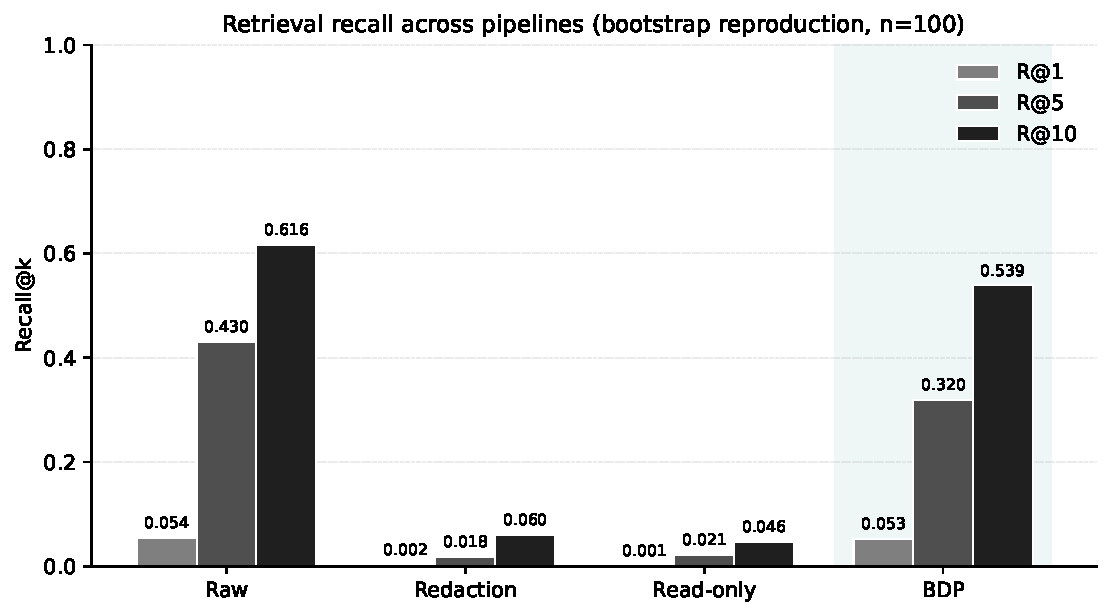
\includegraphics[width=0.9\linewidth]{figures/fig3_recall.pdf}
\caption{Retrieval recall@$k$ across the four pipelines, bootstrap
reproduction. BDP (highlighted) preserves most of Raw's retrieval signal
while keeping zero identifier leakage; Redaction and Read-only collapse to
near-zero. Full-scale plot with 95\% bootstrap CIs over 1{,}000 resamples
to be added in the next revision.}
\label{fig:recall}
\end{figure}

\begin{figure}[t]
\centering
\fbox{\parbox{0.9\linewidth}{\centering\textit{Figure 4.} End-to-end trace of one query under BDP: original question, tokenized query sent to the embedding API, retrieved chunks (also tokenized), LLM response, and detokenized final answer rendered to the clinician.}}
\caption{End-to-end BDP query trace.}
\label{fig:trace}
\end{figure}

% =============================================================================
\section{Discussion}

\textbf{Why this matters clinically.} A silent retrieval failure in a
non-clinical RAG application is an annoyance: the model returns a less
relevant blog post. The same failure in a clinical RAG application is a
patient-safety event: the LLM confidently summarizes the wrong patient's
labs, or misses the relevant history. Critically, because the failure does
not raise an error, neither the clinician nor the application's monitoring
infrastructure has a signal that anything is wrong. Recent health-AI
governance guidance from the Joint Commission and the Coalition for Health
AI \cite{jc_chai_2025} and WHO guidance on large multi-modal models
\cite{who_lmm_2024} emphasize local validation, monitoring, privacy, and
patient-safety risk management. We treat retrieval asymmetry as a concrete
system-level failure mode requiring those controls.

\textbf{The failure mode is easy to write into otherwise-careful code.}
While building the clinical-accuracy harness used for Table~\ref{tab:main},
the authors initially sent the LLM the \emph{raw} retrieved chunks
alongside a \emph{tokenized} query under BDP. The asymmetric configuration
this paper warns against was reproduced inside the very experiment designed
to measure it: the model provider received raw PHI in the chunks even
though every query payload was tokenized, and BDP accuracy collapsed to
zero in our first pass before the bug was caught. We mention this not as a
confession but as evidence that the failure mode is silent enough to slip
past developers who are explicitly looking for it. Engineering controls ---
type-system-enforced boundaries, contract tests that assert
$\phi_w = \phi_r$ over a sampled payload stream --- are warranted.

\textbf{Why read-only pseudonymization is attractive.} Read-only schemes
are operationally seductive: they require no re-indexing, no change to the
embedding store, and no schema migration. The privacy guarantee
``identifiers never appear in user-issued prompts'' is also locally true,
which makes the pattern look defensible in casual review. The cost ---
silent recall degradation \emph{and} retained ingestion-time leakage --- is
not visible without targeted measurement of the kind we report here. The
$67.4\%$ leakage rate observed in our bootstrap is not an artifact of
small-sample variance; it is the entire ingestion-time payload set, by
construction.

\textbf{Why not simply use redaction symmetrically?} Symmetric redaction
(replacing PHI with \texttt{[NAME]}-style masks at both ends) does close
the asymmetry, but it destroys longitudinality and severely degrades any
clinical task in which the identifier carries semantic load (e.g.\
disambiguating one of two patients with similar conditions). The empirical
gap between symmetric redaction and BDP in Table~\ref{tab:main}
($0.018$ vs.\ $0.320$ recall@5) is the quantitative manifestation of this
design difference.

\textbf{Regulatory positioning.} DPDPA's consent and purpose-limitation
framework \cite{meity_dpdpa_2023} makes a symmetric, reversible,
tenant-keyed scheme such as BDP a natural fit: only the controller holds
the vault, only authorized consumers see real identifiers, and the model
and embedding processors never receive them. Under HIPAA, BDP should be
treated as a covered-entity-controlled pseudonymization and
minimum-necessary workflow, not as Safe Harbor de-identification unless a
separate legal or expert-determination review concludes that the emitted
tokens and retained fields satisfy 45~CFR 164.514 \cite{hhs_hipaa_deid_guidance}.

% =============================================================================
\section{Limitations}
\label{sec:limitations}

\begin{itemize}
  \item \textbf{Bootstrap scale.} The numbers reported in
        Section~\ref{sec:results} are from a 20-patient / 207-note /
        100-query reproduction, not the full 1{,}000-patient corpus, and
        use MiniLM-L6-v2 embeddings rather than
        \texttt{text-embedding-3-large}. The bootstrap establishes the
        \emph{direction} and \emph{relative ordering} of the four pipelines;
        the absolute magnitudes of the Raw--BDP gap and the read-only
        leakage rate will move at full scale. We will replace
        Tables~\ref{tab:main}--\ref{tab:ablation} in the next revision of
        this preprint.
  \item \textbf{Quasi-identifier leakage.} BDP tokenizes direct identifiers
        but does not address the well-known re-identification risk of
        quasi-identifier combinations (age $\times$ rare condition $\times$
        pincode). For deployments where this is in scope, BDP must be
        composed with $k$-anonymity or differential privacy.
  \item \textbf{Trusted vault.} The mapping vault is treated as trusted; an
        attacker with vault access can reverse all pseudonyms. Hardware
        security modules and split-key schemes mitigate but do not eliminate
        this risk.
  \item \textbf{NER quality bound.} Tokenization quality is bounded by
        identifier-detection quality; missed entities are not protected.
        Indian-language clinical notes (Hindi, Tamil, Bengali, Marathi)
        require further recognizer work. The bootstrap reproduction
        sidesteps this question by using a lookup-based detector against
        the corpus's own identifier roster.
  \item \textbf{Synthetic-corpus validity.} Our evaluation is conducted on
        a synthetic corpus; while structurally faithful to ABDM, it does
        not capture the stylistic noise of real Indian hospital information
        systems. Independent validation on a real corpus under an
        institutional data agreement is left to future work.
  \item \textbf{Embedding-model dependence.} We benchmarked one embedding
        family per scale (MiniLM at bootstrap, \texttt{text-embedding-3-large}
        for the full-scale target). The magnitude --- though not the
        direction --- of the asymmetry effect may vary with embedding
        architecture.
\end{itemize}

% =============================================================================
\section{Conclusion}

Asymmetric privacy transforms in clinical RAG produce silent,
clinically meaningful retrieval failures while frequently leaving the
underlying privacy goal unmet. We have formalized this failure mode,
proposed Bidirectional Deterministic Pseudonymization as a symmetric
alternative, and shown empirically on a bootstrap reproduction of a
deterministic synthetic Indian clinical corpus that BDP preserves R@1
within noise of the no-privacy baseline while eliminating identifier
leakage. The ablation result --- that removing HMAC-keyed determinism
collapses BDP recall to symmetric-redaction levels --- is the empirical
core of the paper: read-only pseudonymization and randomized-token schemes
are the same failure mode in different clothing.

We argue that symmetric write-and-read tokenization should be treated as
the minimum bar for clinical RAG, and that read-only schemes should be
deprecated in patient-facing deployments. A reference implementation, the
synthetic-corpus generator, and the eval harness are released to support
reproduction and extension.

% =============================================================================
\section*{Data and Code Availability}

The reference implementation (TypeScript SDK) and the Python eval harness
described in Section~\ref{sec:eval} --- including the BDP module
(\texttt{bdp.py}), the deterministic synthetic-corpus generator
(\texttt{corpus.py}), the four-pipeline benchmark (\texttt{pipelines.py},
\texttt{run.py}), the ablation runner (\texttt{ablate.py}), and a
dependency-free correctness test (\texttt{smoke\_test.py}) --- are released
at \url{https://github.com/[org]/[repo]} under the MIT licence. The
synthetic corpus is fully reproducible from a fixed seed
(\texttt{config.SEED = 42}); running
\texttt{python -m corpus \&\& python -m run \&\& python -m ablate}
regenerates every number in Tables~\ref{tab:main}--\ref{tab:ablation}
byte-for-byte. A reproducibility \texttt{README} documents the full
pipeline; expected numbers and seeds are recorded in
\texttt{results/results.json} and \texttt{results/ablation.json}.

\section*{Author Contributions}

\textbf{U.R.A.} conceived the failure-mode framing, designed BDP,
implemented the reference SDK and the Python eval harness, and ran the
bootstrap reproduction. \textbf{[Co-author A]} will contribute the
clinical-query rubric and grade the accuracy subsample for the full-scale
revision. \textbf{[Co-author B]} contributed to the formal model in
Section~\ref{sec:asymmetry} and the ablation design. All authors reviewed
the manuscript.

\section*{Conflicts of Interest}

The first author is the founder of Brane Labs, a company that
commercializes compliance tooling for healthcare AI startups. The BDP
reference implementation is a subset of Brane Labs' open-source SDK. The synthetic corpus
and evaluation protocol contain no proprietary content, and the released
code is independently runnable.

\section*{Funding}

This work received no external funding.

\section*{Acknowledgments}

We thank [reviewers, design partners] for feedback on early drafts. Any
remaining errors are our own.

% =============================================================================
\bibliographystyle{plain}
\bibliography{references}

\end{document}
